\documentclass{article}

%% PAQUETES

% Paquetes generales
\usepackage[margin=2cm, paperwidth=210mm, paperheight=297mm]{geometry}
\usepackage[spanish]{babel}
\usepackage[utf8]{inputenc}
\usepackage{gensymb}

% Paquetes para estilos
\usepackage{textcomp}
\usepackage{setspace}
\usepackage{colortbl}
\usepackage{color}
\usepackage{color}
\usepackage{upquote}
\usepackage{xcolor}
\usepackage{listings}
\usepackage{caption}
\usepackage[T1]{fontenc}
\usepackage[scaled]{beramono}

% Paquetes extras
\usepackage{amssymb}
\usepackage{float}
\usepackage{graphicx}

%% Fin PAQUETES


% Definición de preferencias para la impresión de código fuente.
%% Colores
\definecolor{gray99}{gray}{.99}
\definecolor{gray95}{gray}{.95}
\definecolor{gray75}{gray}{.75}
\definecolor{gray50}{gray}{.50}
\definecolor{keywords_blue}{rgb}{0.13,0.13,1}
\definecolor{comments_green}{rgb}{0,0.5,0}
\definecolor{strings_red}{rgb}{0.9,0,0}

%% Caja de código
\DeclareCaptionFont{white}{\color{white}}
\DeclareCaptionFont{style_labelfont}{\color{black}\textbf}
\DeclareCaptionFont{style_textfont}{\it\color{black}}
\DeclareCaptionFormat{listing}{\colorbox{gray95}{\parbox{16.78cm}{#1#2#3}}}
\captionsetup[lstlisting]{format=listing,labelfont=style_labelfont,textfont=style_textfont}

\lstset{
	aboveskip = {1.5\baselineskip},
	backgroundcolor = \color{gray99},
	basicstyle = \ttfamily\footnotesize,
	breakatwhitespace = true,   
	breaklines = true,
	captionpos = t,
	columns = fixed,
	commentstyle = \color{comments_green},
	escapeinside = {\%*}{*)}, 
	extendedchars = true,
	frame = lines,
	keywordstyle = \color{keywords_blue}\bfseries,
	language = Octave,                       
	numbers = left,
	numbersep = 5pt,
	numberstyle = \tiny\ttfamily\color{gray50},
	prebreak = \raisebox{0ex}[0ex][0ex]{\ensuremath{\hookleftarrow}},
	rulecolor = \color{gray75},
	showspaces = false,
	showstringspaces = false, 
	showtabs = false,
	stepnumber = 1,
	stringstyle = \color{strings_red},                                    
	tabsize = 2,
	title = \null, % Default value: title=\lstname
	upquote = true,                  
}

%% FIGURAS
\captionsetup[figure]{labelfont=bf,textfont=it}

% COMANDOS

%% Titulo de las cajas de código
\renewcommand{\lstlistingname}{Código}
%% Titulo de las figuras
\renewcommand{\figurename}{Figura}
%% Referencia a los códigos
\newcommand{\refcode}[1]{\textit{Código \ref{#1}}}
%% Referencia a las imagenes
\newcommand{\refimage}[1]{\textit{Imagen \ref{#1}}}



\begin{document}

% Inserción del título, autores y fecha.
\title{\huge 61.09 Probabilidad y Estadística \\ 
	  \Huge Trabajo Práctico de Simulación \\
	  \bigskip \Large 13 de mayo de 2012 \\
	  \bigskip \large \textbf{Grupo 1} \\
	  \large \textit{Loiza, Samanta (91935)\\Aguilera, Juan Martín (92483)\\Rossi, Federico Martín (92086)}}
\date{}
\maketitle


% INTRODUCCIÓN

\section{Introducción}

	Con el fin de fortalecer las nociones fundamentales de la probabilidad es que este trabajo busca aplicar las bases de los conceptos ya estudiados en el curso de manera tal de adoptar una mejor comprensión de la inferencia estadística en hechos cotidianos. En este caso, nuestro trabajo será explorar las propiedades estádisticas de cierto tipo de secuencias, las cuales serán detalladas más adelante.
	\par 
	En cada análisis realizado se mostrará su resolución analítica, como así también algoritmos que simulen dichas situaciones, a fin de poder mostrar una aproximación a la constatación empírica de los resultados. Estos últimos se han hecho en el lenguaje de programación \textit{GNU Octave}\footnote{''\textit{GNU Octave} es un lenguaje interpretado de alto nivel, pensado principalmente para cálculos numéricos. Para más información dirijase a \textit{http://www.gnu.org/software/octave} ''}.
	\par 
	Todos los archivos y códigos fuente aquí mencionados, así como también el presente informe, pueden ser descargados de la sección \textit{Downloads} del repositorio del grupo (\textit{http://code.google.com/p/simulacion-proba2012}).



% ACTIVIDADES PREVIAS
\section{Actividades previas}

Tal como lo sugiere el título de este apartado, se mostrarán a continuación una serie de actividades previas necesarias para dominar las técnicas básicas de simulación de números aleatorios.


% ACTIVIDADES PREVIAS - Una primera simulación
\subsection{Una primera simulación}

A continuación, en el \refcode{code:punto1}, se muestra una rutina que, a partir de un generador de números pseudo-aleatorios, permite simular los valores de un dado. Como se puede ver, se ha utilizado la función nativa \textbf{\textit{rand}}, la cual devuelve una matriz (que es utilizada como vector) con valores aleatrios entre 0 y 1. Para ajustarla a nuestras necesidades, o sea, obtener valores aleatorios entre 1 y 6 hemos multiplicado dicho vector por 6. De esta manera pasa a contener valores aleatorios entre 0 y 6. Luego, mediante otra funcion nativa llamada \textbf{\textit{ceil}}, se redondea a los valores enteros próximos superiores de cada uno (ceiling), obteniendo como resultado un vector con valores enteros entre 1 y 6. 

% Código
\lstinputlisting[label=code:punto1,caption=randomDado.m]{source/randomDado.m}

\medskip
\par
Por lo explicado anteriormente, es evidente que como a cada valor se lo trató de la misma manera, se puede decir que no alteramos los resultados del \textbf{\textit{rand}}, y por lo tanto la probabilidad de cada número sigue siendo la misma.

% ACTIVIDADES PREVIAS - Puesta a prueba
\subsection{Puesta a prueba}

Pondremos a prueba ahora lo visto en el apartado anterior estimando las probabilidades de cada uno de los 6 valores posibles utilizando los resultados obtenidos en 1000 ejecuciones de la rutina. [ Colocar contenido aquí ]

\begin{figure}[h]
	\centering
	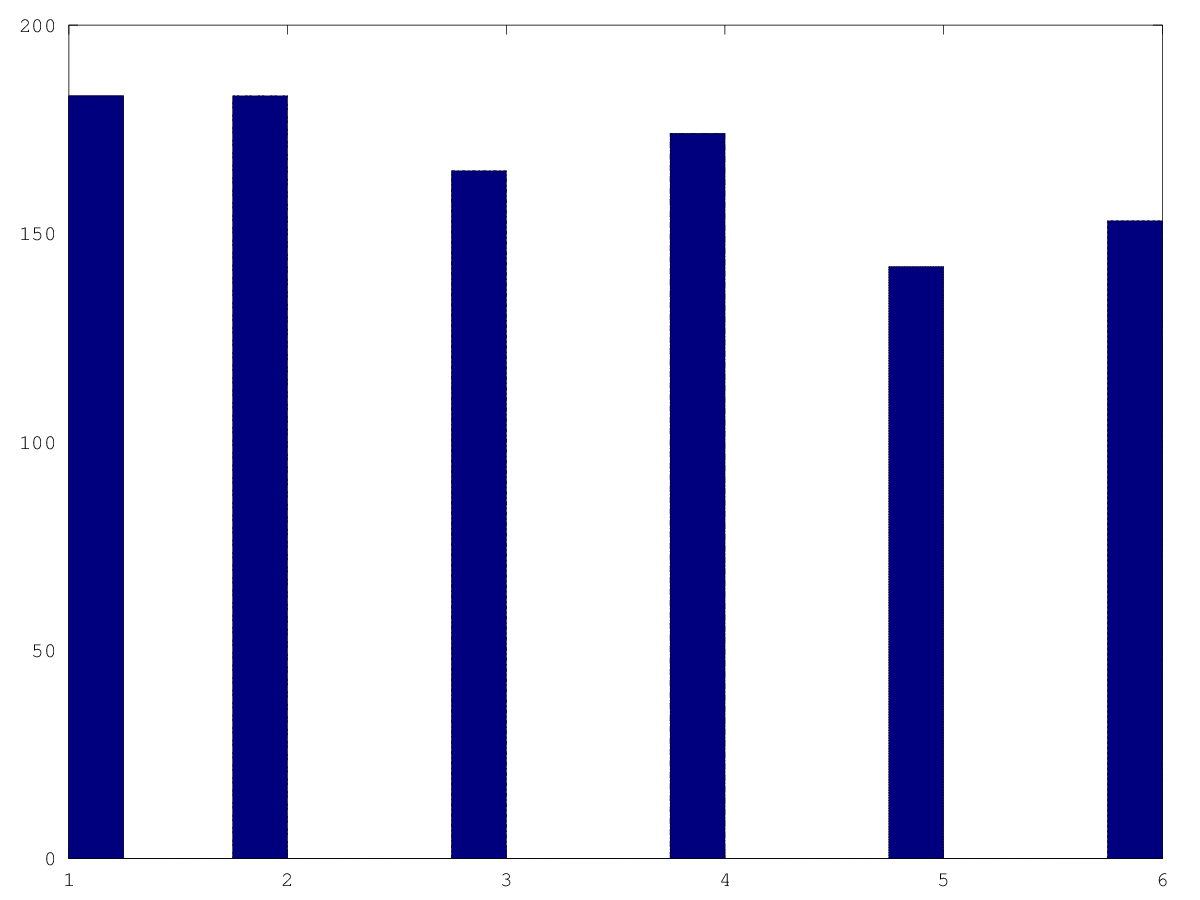
\includegraphics[width=0.50\textwidth]{images/probabilidadesDados.png}
	\caption{Cantidad de veces que sale cada valor de un\\ dado en 1000 lanzamientos de este.}
\end{figure}


% ACTIVIDADES PREVIAS - Predicados
\subsection{Predicados}

A veces se necesita estimar la probabilidad de un evento definido a partir de variables aleatorias. [ Colocar contenido aquí ]

% Código
\lstinputlisting[label=code:punto2,caption=probDobleDelOtro.m]{source/probDobleDelOtro.m}

% ACTIVIDADES PREVIAS - Enigma final
\subsection{Enigma final}

Con lo hecho y aprendido hasta ahora podemos plantearnos la misma pregunta que se hizo a si mismo el Caballero de Méré en el siglo XVII: 

\begin{quotation}
\em``¿Cómo puede ser que cuando apuesto a que voy a obtener al menos un doble as en 24 tiradas de dos dados suelo perder, siendo que suelo ganar cuando apuesto a que voy a obtener al menos un as en 4 tiradas?''
\end{quotation}

\noindent [ Colocar contenido aquí ]

% Código
\lstinputlisting[label=code:punto4.1,caption=probDobleAsEn24Tiradas.m]{source/probDobleAsEn24Tiradas.m}

% Código
\lstinputlisting[label=code:punto4.2,caption=probDobleAs.m]{source/probDobleAs.m}

% ACTIVIDAD PRINCIPAL
\section{Actividad principal}

	Primeramente veamos la situación a analizar. Luego de haber escrito una pieza de software, se desea someterlo a una prueba que garantice su funcionamiento para todas las entradas posibles (finitas). Dado que cada ejecución puede ser afectada por los resultados de las anteriores, se descartan los métodos triviales que consistan en probarlas siguiendo un patrón preestablecido.
	Atendiendo a lo anterior, se propone elegir al azar una entrada con la cual realizar la ejecución y repetir el procedimiento hasta que todas hayan sido elegidas al menos una vez. Si por ejemplo, existen 3 entradas posibles, representadas por los dígitos 1, 2 y 3, las secuencias que se muestran a continuación serían válidas:

\begin{itemize}
\itemsep=2pt \topsep=0pt \partopsep=0pt \parskip=0pt \parsep=0pt
	\item 3 2 2 2 3 3 2 2 3 2 2 2 3 2 3 1
	\item 1 1 2 3
	\item 1 3 2
	\item 2 1 2 2 2 2 3
\end{itemize}

	Es importante remarcar que en cada paso se elige cualquiera sin importar si ya había sido elegida e independientemente de los valores obtenidos anteriormente. Como se puede apreciar, las longitudes de estas secuencias (y por lo tanto, el tiempo y la memoria que consumen) son aleatorias.
	\par 
	Habiendonos situado en lo recién expuesto, pasaremos a explorar y analizar las propiedades estadísticas de las secuencias generadas.
\end{document}
